% Grafica de tiempo frente a talla (el enunciado la pide).
% Lee un CSV por metodo en datos/, que debe generar scripts/bench.py:
%
%   datos/tiempos_ggh_lll_babai.csv        talla,segundos
%                                          2,0.0003
%                                          15,0.016
%
% Cada linea \serie{...} de abajo es un metodo: si su CSV no existe, no se dibuja.
% Mientras no exista el de GGH (LLL + Babai), se muestra un aviso en su lugar.

% \serie{metodo}{estilo de linea}{marca}{leyenda}
\newcommand{\serie}[4]{%
  \IfFileExists{datos/tiempos_#1.csv}{%
    \addplot[black,#2,mark=#3,mark options={solid}]
      table[x=talla,y=segundos,col sep=comma]{datos/tiempos_#1.csv};
    \addlegendentry{#4}}{}}

\IfFileExists{datos/tiempos_ggh_lll_babai.csv}{%
  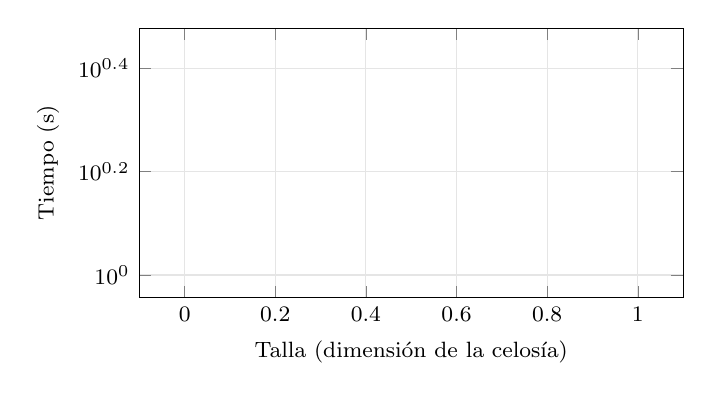
\begin{tikzpicture}
    \begin{semilogyaxis}[
        width=0.7\linewidth,height=5cm,
        xlabel={Talla (dimensión de la celosía)},ylabel={Tiempo (s)},
        font=\footnotesize,
        grid=major,grid style={gray!20},
        legend pos=outer north east,legend cell align=left,
        legend style={draw=none,font=\scriptsize},
        every axis plot/.append style={line width=0.6pt,mark size=1.6pt}]
      \serie{ggh_lll_babai}{solid}{*}{GGH: LLL + Babai}
      \serie{ggh_enumeracion}{solid}{square}{GGH: enumeración}
      \serie{ggh_fuerza_bruta}{solid}{triangle}{GGH: fuerza bruta}
      \serie{lwe_fuerza_bruta}{dashed}{triangle*}{LWE: fuerza bruta}
      \serie{lwe_primal}{dashed}{*}{LWE: ataque primal}
      \serie{ring}{dotted}{diamond*}{Ring-LWE}
    \end{semilogyaxis}
  \end{tikzpicture}%
}{%
  \pendiente{gráfica tiempo frente a talla. Aparece sola cuando existan los CSV de
    \texttt{report/datos/} (formato en \texttt{figuras/tiempos.tex}), generados por
    \texttt{scripts/bench.py}.}%
}
